\section{eo\-Algo$<$ EOT $>$ Class Template Reference}
\label{classeo_algo}\index{eoAlgo@{eoAlgo}}
This is a generic class for population-transforming algorithms.  


{\tt \#include $<$eo\-Algo.h$>$}

Inheritance diagram for eo\-Algo$<$ EOT $>$::\begin{figure}[H]
\begin{center}
\leavevmode
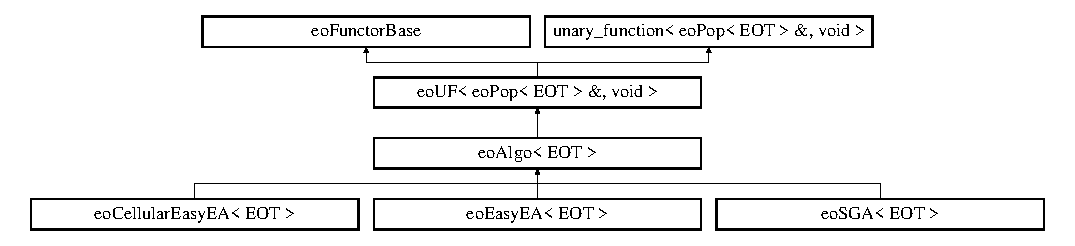
\includegraphics[height=2.86079cm]{classeo_algo}
\end{center}
\end{figure}


\subsection{Detailed Description}
\subsubsection*{template$<$class EOT$>$ class eo\-Algo$<$ EOT $>$}

This is a generic class for population-transforming algorithms. 

There is only one operator defined, which takes a population and does stuff to it. It needn't be a complete algorithm, can be also a step of an algorithm. This class just gives a common interface to linear population-transforming algorithms. 



Definition at line 39 of file eo\-Algo.h.

The documentation for this class was generated from the following file:\begin{CompactItemize}
\item 
eo\-Algo.h\end{CompactItemize}
